\documentclass[10pt,a4paper]{article}
\usepackage[utf8]{inputenc}
\usepackage[T1]{fontenc}
\usepackage[provide=*,spanish]{babel}
\usepackage{lmodern,amsmath,amssymb,booktabs,array,graphicx,xcolor,geometry,fancyhdr,tikz,hyperref}
\usetikzlibrary{arrows.meta,positioning}
\geometry{left=18mm,right=18mm,top=20mm,bottom=19mm}
\definecolor{navy}{HTML}{24465D}
\definecolor{pale}{HTML}{EDF3F7}
\hypersetup{colorlinks=true,urlcolor=navy,linkcolor=navy,pdftitle={Planta geotermica flash-binaria - 230 C y 230 kg/s}}
\setlength{\parindent}{0pt}\setlength{\parskip}{4pt}
\setlength{\abovedisplayskip}{5pt}\setlength{\belowdisplayskip}{5pt}
\pagestyle{fancy}\fancyhf{}
\fancyhead[L]{\small\itshape Centrales termoeléctricas}
\fancyhead[R]{\small Flash + ciclo binario con isobutano}
\fancyfoot[C]{\small\thepage}\renewcommand{\headrulewidth}{0.4pt}
\newcommand{\kj}{\mathrm{kJ/kg}}\newcommand{\su}{\mathrm{kJ/(kg\cdot K)}}
\newcommand{\cs}{\,^{\circ}\mathrm C}
\newcommand{\heading}[1]{\vspace{5pt}{\large\bfseries\color{navy}#1}\par\vspace{2pt}}
\newcommand{\subheading}[1]{\par\vspace{3pt}\textbf{#1}\par}
\newcommand{\note}[1]{\par\vspace{3pt}\noindent\colorbox{pale}{\parbox{\dimexpr\linewidth-2\fboxsep\relax}{#1}}\par\vspace{3pt}}
\newcommand{\xTwo}{0{,}165838}
\newcommand{\sTwo}{2{,}683664}
\newcommand{\mSteam}{38{,}143}
\newcommand{\mBrine}{191{,}857}
\newcommand{\hFour}{2344{,}540}
\newcommand{\QHX}{50{,}480}
\newcommand{\mIso}{105{,}535}
\newcommand{\hEight}{754{,}305}
\newcommand{\hNine}{690{,}061}
\newcommand{\hTen}{270{,}174}
\newcommand{\sTen}{1{,}242431}
\newcommand{\TTen}{29{,}565}
\newcommand{\vTen}{0{,}00183517}
\newcommand{\hEleven}{275{,}985}
\newcommand{\wPump}{5{,}81138}
\newcommand{\WFlash}{15{,}412}
\newcommand{\WTIso}{6{,}780}
\newcommand{\WPump}{0{,}613}
\newcommand{\WBinary}{6{,}167}
\newcommand{\WTotal}{21{,}579}
\newcommand{\QFlash}{97{,}522}
\newcommand{\QIn}{148{,}002}
\newcommand{\QGeo}{148{,}001}
\newcommand{\QCFlash}{82{,}110}
\newcommand{\QCIso}{44{,}313}
\newcommand{\QResource}{203{,}589}
\newcommand{\etaBinary}{12{,}216}
\newcommand{\etaCombined}{14{,}580}
\newcommand{\etaTwenty}{10{,}354}
\newcommand{\etaResource}{10{,}599}
\newcommand{\stateRows}{%
1 & Agua & 27{,}951 & 230{,}000 & 990{,}000 & 2{,}609710 & 230{,}000 \\
2 & Agua & 5{,}000 & 151{,}866 & 990{,}000 & 2{,}683664 & 230{,}000 \\
3 & Agua & 5{,}000 & 151{,}866 & 2748{,}600 & 6{,}821400 & 38{,}143 \\
4 & Agua & 0{,}100 & 45{,}817 & 2344{,}540 & 7{,}398360 & 38{,}143 \\
5 & Agua & 0{,}100 & 45{,}817 & 191{,}830 & 0{,}649260 & 38{,}143 \\
6 & Agua & 5{,}000 & 151{,}866 & 640{,}380 & 1{,}861040 & 191{,}857 \\
7 & Agua & 5{,}000 & 90{,}000 & 377{,}270 & 1{,}192220 & 191{,}857 \\
8 & Isobutano & 32{,}500 & 145{,}000 & 754{,}305 & 2{,}527984 & 105{,}535 \\
9 & Isobutano & 4{,}000 & 80{,}000 & 690{,}061 & 2{,}605089 & 105{,}535 \\
10 & Isobutano & 4{,}000 & 29{,}565 & 270{,}174 & 1{,}242431 & 105{,}535 \\
11 & Isobutano & 32{,}500 & --- & 275{,}985 & --- & 105{,}535 \\
}

\begin{document}
\begin{center}
{\small\bfseries ESCUELA PROFESIONAL DE INGENIERÍA MECÁNICA ELÉCTRICA}\\[4pt]
{\Large\bfseries\color{navy}Planta geotérmica flash-binaria}\\[3pt]
{\large Recurso a $230\cs$, caudal $230\ \mathrm{kg/s}$}\\[2pt]
{\small Desarrollo de los tres apartados de la fotografía}
\end{center}
\heading{1. Datos e interpretación del esquema}
\begin{center}\small
\begin{tabular}{lll}\toprule
Condición&Estado o símbolo&Valor\\\midrule
Agua del pozo, líquido saturado&1&$T_1=230\cs$, $\dot m_1=230\ \mathrm{kg/s}$\\
Expansión flash isoentálpica&$1\to2$&$p_2=500\ \mathrm{kPa}=5$ bar\\
Salida de turbina de vapor&4&$p_4=10\ \mathrm{kPa}$, humedad 10\,\%\\
Salida geotérmica del intercambiador&7&$T_7=90\cs$\\
Entrada de turbina de isobutano&8&$p_8=3{,}25\ \mathrm{MPa}$, $T_8=145\cs$\\
Salida de turbina de isobutano&9&$p_9=400\ \mathrm{kPa}$, $T_9=80\cs$\\
Condensador del isobutano&$9\to10$&$p_{10}=400\ \mathrm{kPa}$\\
Eficiencia isentrópica de la bomba&$10\to11$&$\eta_B=0{,}90$; $p_{11}=3{,}25\ \mathrm{MPa}$\\\bottomrule
\end{tabular}
\end{center}
\textbf{Humedad del 10\,\% significa calidad de vapor $x_4=1-0{,}10=0{,}90$.} Los $80\cs$ corresponden al escape de la turbina de isobutano, no a la salida de su condensador.

\begin{center}
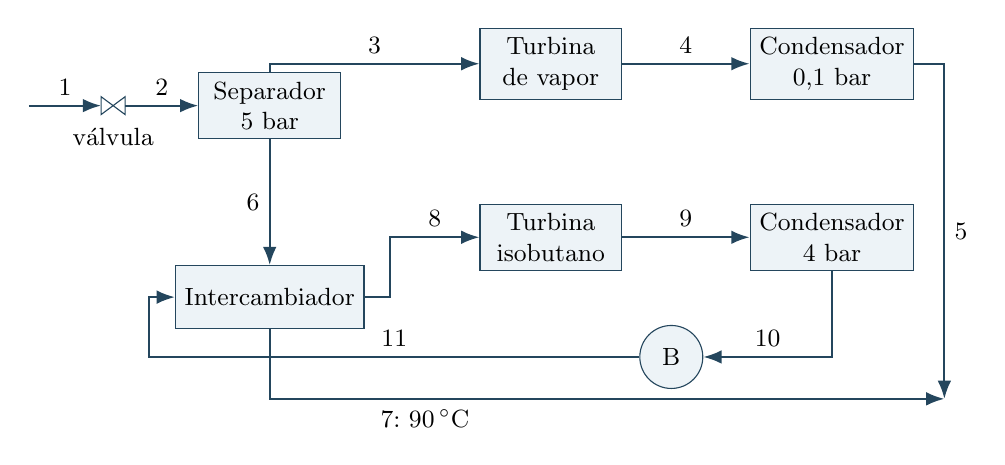
\begin{tikzpicture}[x=1.02cm,y=.76cm,>=Latex,every node/.style={font=\small},box/.style={draw=navy,fill=pale,align=center,minimum width=1.8cm,minimum height=.8cm},pipe/.style={->,thick,draw=navy}]
\node[box] (S) at (0,2) {Separador\\5 bar};
\node[box] (T) at (3.5,2.7) {Turbina\\de vapor};
\node[box] (C) at (7,2.7) {Condensador\\0,1 bar};
\node[box] (HX) at (0,-1.2) {Intercambiador};
\node[box] (IT) at (3.5,-.2) {Turbina\\isobutano};
\node[box] (IC) at (7,-.2) {Condensador\\4 bar};
\node[circle,draw=navy,fill=pale,minimum size=8mm] (P) at (5,-2.2) {B};
\draw[pipe] (-3,2)--node[above]{1}(-2.1,2);
\draw[navy] (-2.1,1.85)--(-1.8,2.15)--(-1.8,1.85)--(-2.1,2.15)--cycle;
\node[below] at (-1.95,1.78) {válvula};
\draw[pipe] (-1.8,2)--node[above]{2}(S.west);
\draw[pipe] (S.north)--(0,2.7)--node[above]{3}(T.west);
\draw[pipe] (T.east)--node[above]{4}(C.west);
\draw[pipe] (C.east)--(8.4,2.7)--node[right]{5}(8.4,-2.9);
\draw[pipe] (S.south)--node[left]{6}(HX.north);
\draw[pipe] (HX.south)--(0,-2.9)--node[pos=.23,below]{7: $90\cs$}(8.4,-2.9);
\draw[pipe] (HX.east)--(1.5,-1.2)--(1.5,-.2)--node[above]{8}(IT.west);
\draw[pipe] (IT.east)--node[above]{9}(IC.west);
\draw[pipe] (IC.south)--(7,-2.2)--node[above]{10}(P.east);
\draw[pipe] (P.west)--node[above]{11}(-1.5,-2.2)--(-1.5,-1.2)--(HX.west);
\end{tikzpicture}
\end{center}
\textbf{Modelo:} operación estacionaria; separador y válvula ideales; intercambiador sin pérdidas; caídas de presión y variaciones cinética/potencial despreciables. Ambos condensadores entregan líquido saturado. No se indican consumos de ventiladores, bombas geotérmicas ni pérdidas de generador; la potencia neta binaria incluye la bomba indicada.

\heading{2. Agua: separación y potencia flash}
Del repositorio de tablas: $h_1=h_f(230\cs)=990{,}00$, $h_3=h_g(5\ \mathrm{bar})=2748{,}60$, $h_6=h_f(5\ \mathrm{bar})=640{,}38$ y $h_{fg}(5\ \mathrm{bar})=2108{,}2\ \kj$.
\begin{align*}
h_2&=h_1,\qquad
x_2=\frac{990{,}00-640{,}38}{2108{,}2}=\xTwo,\\
\dot m_3&=230x_2=\boxed{\mSteam\ \mathrm{kg/s}},\qquad
\dot m_6=230-\dot m_3=\boxed{\mBrine\ \mathrm{kg/s}},\\
h_4&=h_f(0{,}1)+0{,}90h_{fg}(0{,}1)=191{,}83+0{,}90(2391{,}9)=\hFour\ \kj,\\
\dot W_{flash}&=\dot m_3(h_3-h_4)
=\frac{\mSteam(2748{,}60-\hFour)}{1000}
=\boxed{\WFlash\ \mathrm{MW}}.
\end{align*}
La división entre 1000 convierte kW en MW. Se desprecia el trabajo auxiliar de la sección flash por no estar especificado.

\newpage
\heading{3. Propiedades del isobutano y trabajo de la bomba}
Se utilizan las cuatro páginas de \textbf{tablas.pdf, R-600a (isobutano)}, aportadas por el usuario. Las columnas $0,5,\ldots,100\cs$ de las páginas 2--4 indican \textbf{sobrecalentamiento} $\Delta T=T-T_{sat}$.
\subheading{Interpolación de las entalpías de vapor (página 3)}
Para $p_8=32{,}5$ bar y $T_8=145\cs$, las filas vecinas son $(30{,}880\ \mathrm{bar},125\cs)$ y $(33{,}578\ \mathrm{bar},130\cs)$. Sus sobrecalentamientos son 20 y 15 °C, respectivamente:
\[
h_8=761{,}181+\frac{32{,}5-30{,}880}{33{,}578-30{,}880}(749{,}729-761{,}181)
=\boxed{\hEight\ \kj}.
\]
Para $p_9=4$ bar y $T_9=80\cs$, las filas son $(3{,}507\ \mathrm{bar},25\cs)$ y $(4{,}047\ \mathrm{bar},30\cs)$: $\Delta T=55$ y $50\cs$.
\[
h_9=691{,}396+\frac{4-3{,}507}{4{,}047-3{,}507}(689{,}934-691{,}396)
=\boxed{\hNine\ \kj}.
\]
\subheading{Líquido saturado a la entrada de la bomba (página 1)}
La fracción de interpolación es $f=(4-3{,}507)/(4{,}047-3{,}507)=0{,}912963$.
\begin{align*}
h_{10}&=258{,}980+f(271{,}241-258{,}980)=\hTen\ \kj,\\
v_{10}&=\frac{1{,}816+f(1{,}837-1{,}816)}{1000}=\vTen\ \mathrm{m^3/kg},\\
T_{10}&=25+5f=\TTen\cs,\qquad s_{10}=1{,}205+f(1{,}246-1{,}205)=\sTen\ \su.
\end{align*}
El volumen líquido está impreso en dm$^3$/kg: se divide entre 1000 para usarlo con presiones en kPa.
\subheading{Bomba: aproximación de líquido incompresible}
\begin{align*}
w_B&\simeq\frac{v_{10}(p_{11}-p_{10})}{\eta_B}
=\frac{\vTen(3250-400)}{0{,}90}=\boxed{\wPump\ \kj},\\
h_{11}&=h_{10}+w_B=\boxed{\hEleven\ \kj}.
\end{align*}
Estas tablas no incluyen líquido comprimido de isobutano. Por ello se declara esta aproximación y no se asignan $T_{11}$ ni $s_{11}$. No se supone que la bomba real sea isentrópica.

\heading{4. Apartado 1: flujo másico de isobutano}
El agua que calienta el isobutano es \textbf{solo el líquido del separador}, $\dot m_6=\mBrine\ \mathrm{kg/s}$. A la salida geotérmica se usa la propiedad de líquido comprimido a 5 bar y 90 °C: $h_7=377{,}27\ \kj$.
\begin{align*}
\dot Q_{HX}&=\dot m_6(h_6-h_7)
=\frac{\mBrine(640{,}38-377{,}27)}{1000}=\QHX\ \mathrm{MW},\\
\dot m_6(h_6-h_7)&=\dot m_{iso}(h_8-h_{11}),\\
\boxed{\dot m_{iso}}&=\frac{\dot m_6(h_6-h_7)}{h_8-h_{11}}
=\frac{\mBrine(640{,}38-377{,}27)}{\hEight-\hEleven}
=\boxed{\mIso\ \mathrm{kg/s}}.
\end{align*}
Usar $h_7\simeq h_f(90\cs)=376{,}93\ \kj$ es una aproximación habitual; aquí se conserva el valor de líquido comprimido que está disponible en las tablas.

\heading{5. Apartado 2: potencia neta binaria y total}
\begin{align*}
\dot W_{T,iso}&=\dot m_{iso}(h_8-h_9)
=\frac{\mIso(\hEight-\hNine)}{1000}=\WTIso\ \mathrm{MW},\\
\dot W_B&=\dot m_{iso}w_B=\WPump\ \mathrm{MW},\\
\boxed{\dot W_{n,bin}}&=\dot W_{T,iso}-\dot W_B
=\WTIso-\WPump=\boxed{\WBinary\ \mathrm{MW}},\\
\boxed{\dot W_{n,total}}&=\dot W_{flash}+\dot W_{n,bin}
=\WFlash+\WBinary=\boxed{\WTotal\ \mathrm{MW}}.
\end{align*}

\newpage
\heading{6. Apartado 3: eficiencias térmicas}
\subheading{Ciclo binario}
\[
\boxed{\eta_{bin}=\frac{\dot W_{n,bin}}{\dot Q_{HX}}
=\frac{\WBinary}{\QHX}=\etaBinary\,\%}.
\]
\subheading{Planta combinada: recurso respecto al ambiente estándar}
El ejercicio original equivalente, problema 141 del capítulo 23 de \emph{Fundamentals of Thermal-Fluid Sciences}, remite a la definición del problema 139: energía del recurso respecto al ambiente estándar. Para seguir ese criterio se declara $T_0=25\cs$ y $h_0\simeq h_f(25\cs)=104{,}83\ \kj$. La temperatura ambiental no está escrita en la fotografía.
\begin{align*}
\dot E_{geo,25}&=\dot m_1(h_1-h_0)
=\frac{230(990{,}00-104{,}83)}{1000}=\QResource\ \mathrm{MW},\\
\boxed{\eta_{comb}}&=\frac{\dot W_{n,total}}{\dot E_{geo,25}}
=\frac{\WTotal}{\QResource}=\boxed{\etaResource\,\%}.
\end{align*}
\note{\textbf{Otra base térmica.} La energía efectivamente retirada del geofluido es $\dot Q_{ret}=\dot m_3(h_3-h_5)+\dot Q_{HX}=\QIn\ \mathrm{MW}$, con $h_5=191{,}83\ \kj$. Dividir la potencia entre esa cantidad da $\eta_{ret}=\etaCombined\,\%$. Es un denominador diferente del recurso respecto al ambiente. Para $T_0=20\cs$ el rendimiento del recurso sería $\etaTwenty\,\%$.}

\heading{7. Tabla completa de estados}
\begin{center}\small
\setlength{\tabcolsep}{4pt}\renewcommand{\arraystretch}{1.23}
\begin{tabular}{clrrrrr}\toprule
Estado&Fluido&$p$ (bar)&$T$ ($^\circ$C)&$h$ ($\kj$)&$s$ ($\su$)&$\dot m$ (kg/s)\\\midrule
\stateRows
\bottomrule
\end{tabular}
\end{center}
Los estados 1, 5 y 6 son líquido saturado; 2 es mezcla tras la válvula; 3 es vapor saturado; 4 es mezcla con $x_4=0{,}90$; 7 es líquido comprimido. En el isobutano, 8 y 9 son vapor sobrecalentado, 10 líquido saturado y 11 líquido comprimido. Las referencias de entalpía de fluidos diferentes no se mezclan en los balances.

\subheading{Comprobación de energía}
\[
\dot Q_{C,vapor}=\QCFlash\ \mathrm{MW},\qquad
\dot Q_{C,iso}=\QCIso\ \mathrm{MW},\qquad
\dot Q_{ret}=\dot W_{n,total}+\dot Q_{C,vapor}+\dot Q_{C,iso}.
\]
Los balances de la bomba, intercambiador y ambos ciclos cierran con los valores sin redondear. La expresión global $\dot m_1h_1-\dot m_5h_5-\dot m_7h_7\simeq\QGeo\ \mathrm{MW}$ difiere en menos de 1 kW por los redondeos de $h_f$, $h_g$ y $h_{fg}$ de las tablas de agua.

{\footnotesize\raggedright\textbf{Fuentes.} Fotografía del usuario; agua: \href{https://github.com/dilmar231gabriel-ops/Tablas.KchaParedes}{Tablas.KchaParedes}; isobutano: tablas.pdf del usuario, páginas 1--4, digitalizadas en \href{https://github.com/Aquiles-ryp360/Tablas.KchaParedesbykiles/tree/main/data/r600a}{su repositorio GitHub}. Contraste: \href{https://www.rose-hulman.edu/ES202/Chapter\%2023\%20of\%20Text/chapter23.pdf}{capítulo 23, problemas 139 y 141}, texto alojado por Rose-Hulman. La clave del libro publica 105,5 kg/s, 15,4 MW, 6,14 MW, 12,2\,\% y 10,6\,\%, con propiedades EES. El desarrollo actual utiliza las tablas R-600a aportadas y las tablas de agua del repositorio. Las pequeñas diferencias se deben a las propiedades y a la aproximación de la bomba.\par}
\end{document}
